\subsection{Level2.1: $y=x^2$}
\subsubsection{プログラムソース}
\lstinputlisting[caption=変更された関数f(x\,y),label=ラベル]{./figs/f2-1.txt}
\lstinputlisting[caption=変更されたf(x\,y)の微分値,label=ラベル]{./figs/x2-1.txt}
\subsubsection{観察意図と観察方法(実験計画)}
変更したプログラムに対して、シード値を1、α値を0.1として実行する。run\_ave.shファイルの実行結果により、シード値が及ぼす挙動についてみれるはずなので、その結果をもとにシード値の考察を行う。次にα値により探索点の推移距離が変わるので、シード値を固定したままα値をより大きく、または小さくした値に変更して実験を行うことでα値が探索挙動に及ぼす影響を考察する。この時、関数に対して谷が1つなのでxの解やα値が1つに定まるはずなのでそれを意識する。
\subsubsection{実行結果}
\lstinputlisting[caption=\.\/steepest\_decent 1の実行結果,label=ラベル]{./figs/hoge2-1.txt}
シード値を1、α値を0.1に設定して実行した結果、xの値が-7.3692442371から始まり、step63でf(x)の値が0、
探索点がほとんど動かなくなった為step75で終了した。\\
./run\_ave.shを用いてシード値を千刻み10パターン(1000〜10000)で実行し平均試行回数を計測した。1000〜10000までそれぞれの試行回数は順に64、75、69、74、71、73、73、72、74、70であり、平均試行回数は71.5stepであった。
\newline
\begin{figure}[htbp]
  \begin{center}
    \begin{tabular}{c}

      % 1
      \begin{minipage}{0.5\hsize}
        \begin{center}
          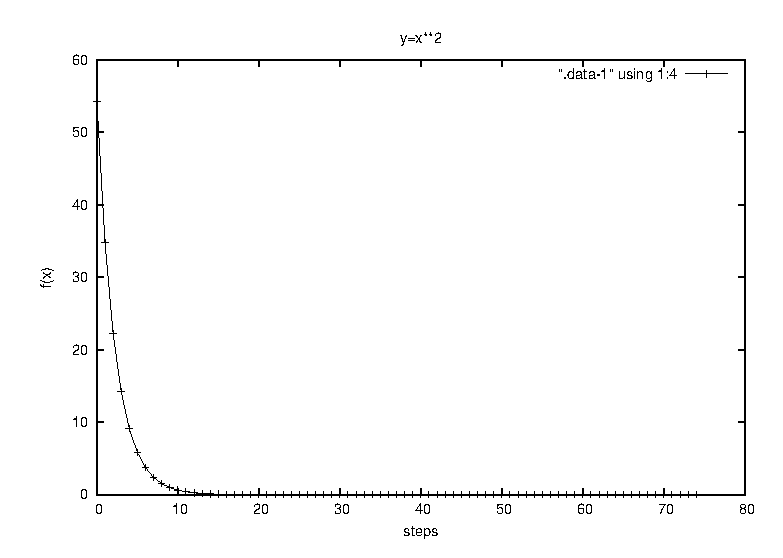
\includegraphics[clip, width=7cm]{./figs/sim2-1_step-1.eps}
          \hspace{1.6cm} 図1 stepあたりの目的関数推移線グラフ
        \end{center}
      \end{minipage}

      % 2
      \begin{minipage}{0.5\hsize}
        \begin{center}
          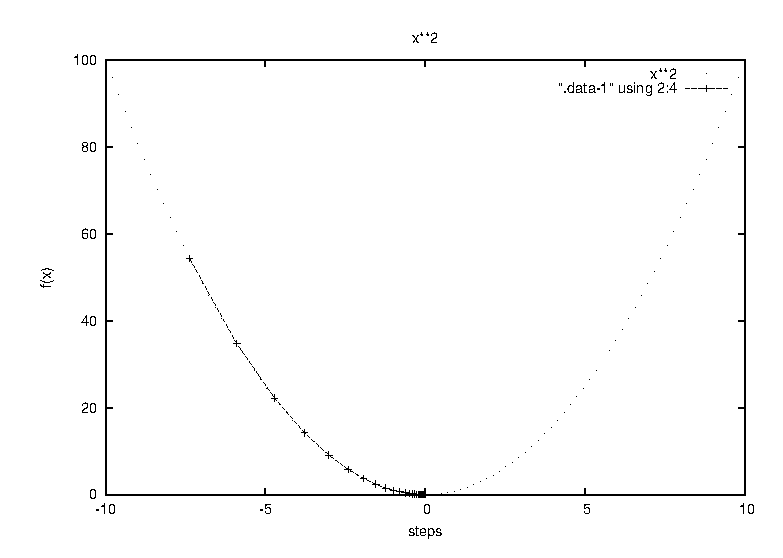
\includegraphics[clip, width=7cm]{./figs/sim2-1-1.eps}
          \hspace{1.6cm} 図2 探索点が関数上をどのように推移したかを示すグラフ
        \end{center}
      \end{minipage}

    \end{tabular}
  \end{center}
\end{figure}
\newline
図1と図2はシード値1、αを0.1に設定して実行された最急降下法アルゴリズムにおける点のstepあたりの移線グラフと関数上での推移グラフである。
\subsubsection{考察}
シード値は探索点の初期値の設定に用いるものである。実験結果よりシード値による高さの決定はランダムであるが、α値を固定した場合は、決定した高さがより低いほうがstep数は少ない事が分かった。さらにコマンド「tail -1 .archive-*」を実行した結果、高さと得られる解の質は関係がないと考えられた。\\
α値に関しての考察を得るためシード値1、α値0.1における実験に対してα値を変更した2つの実験を行う。シード値を固定したままα値を0.3、0.007に変更する。シード値は固定であるため開始地点は同じになる。
\lstinputlisting[caption=α値0.3、0.007に置ける\.\/steepest\_decent 1の実行結果,label=ラベル]{./figs/huga2-1.txt}
\begin{figure}[htbp]
  \begin{center}
    \begin{tabular}{c}

      % 1
      \begin{minipage}{0.5\hsize}
        \begin{center}
          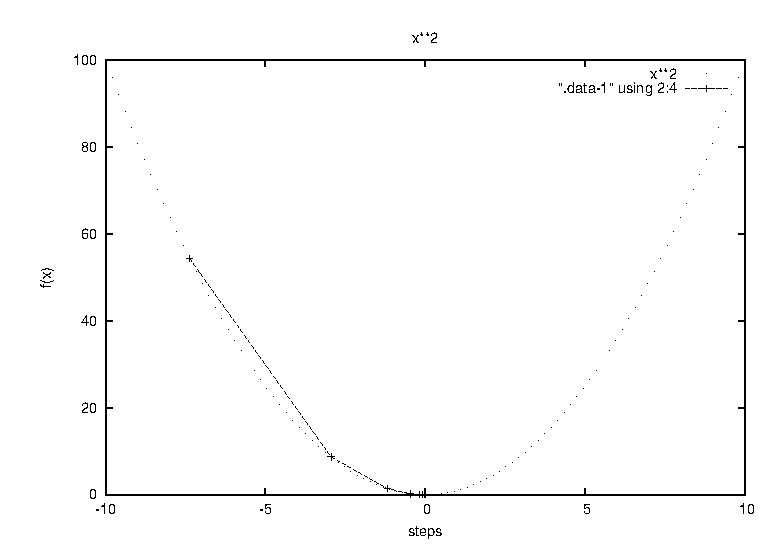
\includegraphics[clip, width=7cm]{./figs/sim2-1-0_3.eps}
          \hspace{1.6cm} 図3 探索点の関数上での推移を示すグラフ(α値0.3)
        \end{center}
      \end{minipage}

      % 2
      \begin{minipage}{0.5\hsize}
        \begin{center}
          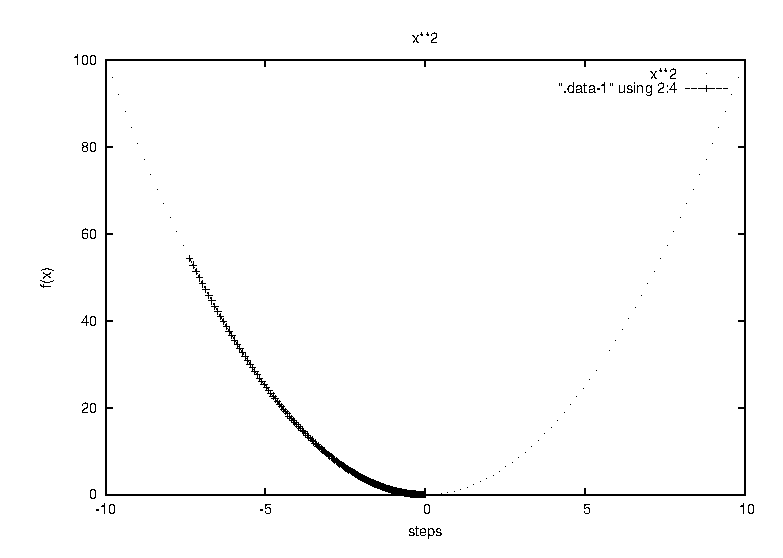
\includegraphics[clip, width=7cm]{./figs/sim2-1-0_007.eps}
          \hspace{1.6cm} 図4 探索点の関数上での推移を示すグラフ(α値0.007)
        \end{center}
      \end{minipage}

    \end{tabular}
  \end{center}
\end{figure}
α値を変更する事で推移距離が変わる。α値を0.3にすると推移距離が長くなり、小さくすると短くなる。
α値を0.3にすると、α値0.007、0.1に比べ、step21で探索が済んでいるため効率性がよく、得られる解の質に関しても、誤差が小さくなっていることが実行結果より判断出来る。
α値を小さくすると誤差がより大きくなってしまったことに関しては、小さいと探索点から動いていないと判断されてしまい、探索を打ち切られてしまうからと考えられる。\\
これらの実行結果より、3つのα値の内0.3付近がより、探索における有用性が見いだせる。今回の場合、最小値の値が0であり、傾きの値が0となる点であることが自明である。よって移動先の算出は式から見いだせ、その値はα値が0.5のときである。つまりα値が0.5の時step2で最適値を見つけ出す事ができ、解の質においても誤差はない。今回の実験で、0.3付近でより有用性が見いだせたのは、より0.5に近かったからと判断できる。

